\chapter{Descrizione plug-in: un manuale d'uso}
\label{sec:plugindesc}
Le operazioni compiute dal software qui descritto si dividono sostanzialmente in tre parti:
\begin{itemize}
  \item una prima parte di \emph{configurazione}
  \item una parte di \emph{precalcolo}
  \item una parte di \emph{customizzazione} dei risultati tramite l'utilizzo di varie opzioni fornite dalla \emph{GUI}
\end{itemize}
In questo capitolo si vogliono descrivere le funzionalit� a disposizione dell'utente, nell'utilizzo del \emph{plug-in}, sia in fase di configurazione che in fase di presentazione e analisi dei risultati, mentre la parte di calcolo verr� descritta pi� approfonditamente nel capitolo \ref{sec:internalfunct} alla luce dei parametri utilizzati e presentati.\\




	
	\section{Selezione dell'intervallo temporale da analizzare}
	\label{sec:audioselection}
		Prima di lanciare il \emph{plug-in}, � necessario caricare il file audio della registrazione multicanale acquisita con l'\emph{array microfonico} nell'host \audacity. 
		
		Di tutta la registrazione, che pu� in alcuni casi durare anche qualche ora, potrebbe essere necessario selezionare solo una parte, in modo da focalizzarsi nell'analisi su un particolare intervallo di tempo, all'occorrenza anche molto breve. 		
		%%%%%%%%%%%%%%%%%%%%%%%%%%%%%%%% FIGURA AUDIO SELECTION %%%%%%%%%%%%%%%%%%%%%%%%%%%%
\begin{figure}
  \centering
  \includegraphics[width = 12cm]{img/audioselect.png}
  \caption{Selezione dello spezzone di materiale audio da analizzare con il \emph{plug-in}.\\}
  \label{fig:audioselect}
\end{figure}
		Si pensi per esempio all'analisi delle prime riflessioni in una sala da concerto: in questo tipo di studio, si � interessati al comportamento di un ambiente sotto l'aspetto degli echi e altri effetti.
		A questo scopo � necessario selezionare la porzione di audio di interesse, come indicato in figura \ref{fig:audioselect}. 
		Cos� facendo si limita il materiale audio che \audacity deve editare attraverso i \emph{plug-in} (denominati \emph{effects}).
		
		
				%%%%%%%%%%%%%%%%%%%%%%%%%%%%%%%% FIGURA OUTOFMEMORY %%%%%%%%%%%%%%%%%%%%%%%%%%%%
\begin{figure}
  \centering
  \includegraphics[width = 12cm]{img/outofmemory.png}
  \caption{Messaggio di errore in caso di memoria insufficiente per le operazioni di \emph{precalcolo}\\}
  \label{fig:outofmemory}
\end{figure}

		In alternativa � possibile selezionare anche l'intera registrazione, ben sapendo che l'analisi compiuta nel \emph{precalcolo} � computazionalmente molto onerosa, nonch� esigente per quanto riguarda l'utilizzo delle \emph{risorse}, perci� va incontro alla possiblit� che in questa fase il programma si interrompa prima di aver analizzato tutti i frame.
		In tal caso verr� presentato un messaggio di avviso, come da figura \ref{fig:outofmemory}, e il programma passer� alla visualizzazione dei soli risultati analizzati fino a quel momento.
		Si tenga presente che su un normale laptop con processore \emph{dual core} da $2.0 \; GHz$ con $2\;GB$ di $RAM$, l'elaborazione pi� lunga complessivamente effettuabile consta di circa $60$ frames e impiega circa 90 secondi per il \emph{precalcolo}.
		
		Sar� sempre possibile costruire un video a partire dai singoli frames esportati in diverse elaborazioni del plug-in, operando su spezzoni audio consecutivi. \\
		
		
		
		
	\section{Finestra di configurazione}
	\label{sec:confdlg}
		Una volta selezionato il materiale audio da analizzare, dal menu \emph{Effect} di \audacity \; � possibile accedere al \emph{plug-in} in oggetto, alla voce \emph{Microphone Array Analyzer}. 
		
						%%%%%%%%%%%%%%%%%%%%%%%%%%%%%%%% FIGURA CONFIGURATION DIALOG %%%%%%%%%%%%%%%%%%%%%%%%%%%%
\begin{figure}
  \centering
  \includegraphics[width = 12cm]{img/confdlgBIG.png}
  \caption{Finestra di configurazione del modulo \emph{Microphone Array Analyzer}\\}
  \label{fig:confdlg}
\end{figure}
		
		La prima finestra che appare all'utente � mostrata in figura \ref{fig:confdlg}. 
		Si tratta di una finestra di dialogo dedicata all'inserimento di alcuni parametri per l'analisi del materiale audio precedentemente selezionato. 
		
		Attraverso questa finestra l'utente dovr� specificare:
		\begin{description}
		  \item [Un \textbf{videoclip dell'ambiente di background}] acquisito, con una videocamera adatta allo scopo\footnote{\;Per una descrizione delle telecamere nei singoli array si ritorni al capitolo \ref{sec:array} }, durante la registrazione dell'evento sonoro, su cui mappare i livelli \emph{SPL} con le bande di colore.
		  \item [Un\textbf{ file di configurazione }] in formato \emph{xml}  contenente la mappatura in \emph{pixel} delle posizioni delle singole capsule microfoniche sulla immagine di background.
		  Il file contiene anche una serie di informazioni sull'array stesso, come nome e tipologia, casa produttrice ecc, 
		  \item [Il livello di trasparenza] della colormap al sovrapporsi al video di background.
		  \item [il livello min SPL] cio� il limitie inferiore della scala di $dB$ che si vuole analizzare. 	
		  I pixel eventualmente presenti nella \emph{color-map} con valori SPL che non superassero questa soglia verrebbero disegnati completamente trasparenti.
		  \item[livello di fondo scala FS] utile per effettuare una sorta di taratura che adeguer� verso quel limite tutti gli altri valori misurati per dare loro una verosimiglianza fisica.
		  \item [frame length] dello spezzone audio elementare in cui si vuole suddividere il materiale importato per effettuarne l'analisi. Corrisponde alla lunghezza del frame del video finale di output.
		  \item [frame overlap] cio� la percentuale con cui ogni frame si sovrappone nel tempo a quello a lui immediatamente precedente in modo da aggiungere un certo grado di \emph{smoothing} per controbilanciare l'operazione di finestratura\footnote{\; Descritta al capitolo \ref{sec:windowing}} svolta dal \emph{plug-in} in seguito alla suddivisione del materiale di analisi.
		\end{description}		
		La coerenza dei dati verr� verificata automaticamente e, in caso di rilevamento di incongruenze, verr� visualizzato un messaggio di errore con una breve spiegazione.\\

		
		
	
	\section{Interfaccia principale}
	\label{sec:MAAdlg}
	%%%%%%%%%%%%%%%%%%%%%%%%%%%%%%%% FIGURA MAA DIALOG %%%%%%%%%%%%%%%%%%%%%%%%%%%%
\begin{figure}
  \centering
  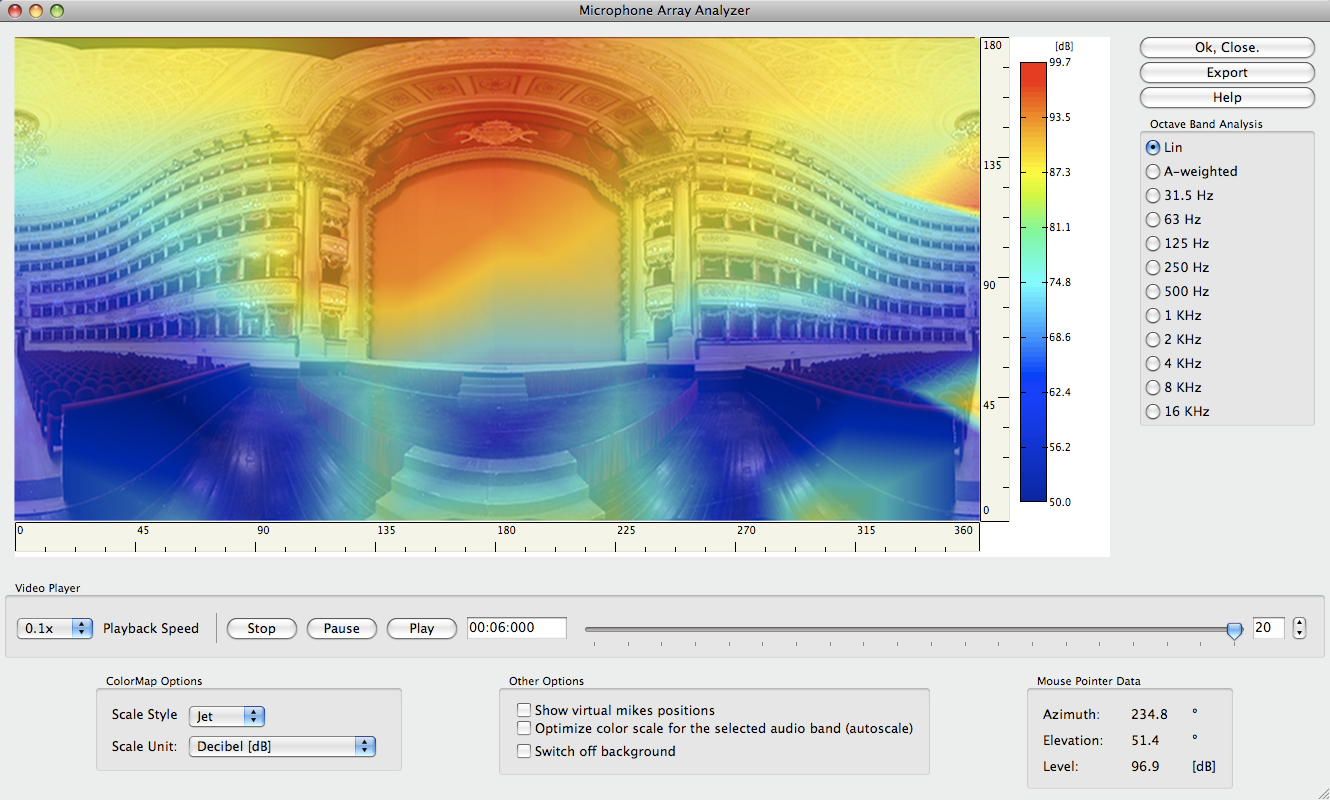
\includegraphics[width = 12cm]{img/maadlg.png}
  \caption{Finestra principale del modulo \emph{Microphone Array Analyzer}\\}
  \label{fig:maadlg}
\end{figure}
	Come possiamo notare in figura \ref{fig:maadlg}, la finestra principale del \emph{plug-in} mostra un video player contenente un video di output preliminare, ottenuto utilizzando un set di opzioni di default. 
	Si ha per� accesso anche a tutte queste opzioni direttamente dagli altri pannelli della finestra, potendo quindi modificare ciascuna di queste opzioni e di conseguenza il video di output.
	Si procede ora con la descrizione, una per una, di queste configurazioni ulteriormente disponibili:
		\begin{description}
 		 \item[Selettore di banda di frequenze] secondo cui filtrare i risultati e osservare quindi al meglio il comportamento delle onde sonore in una banda particolare. 
		 Si pu� quindi discriminare l'emissione di energia sonora in una particolare regione di spettro.
		 Questo tipo di analisi pu� essere molto utile quando si cerca di studiare un campo acustico dovendo discriminare diverse sorgenti sonore o particolari riflessioni di uno stesso impulso. Grazie al \emph{filtro passa-banda} � possibile eliminare dall'analisi del campo acustico tutto il materiale sonoro di minor interesse evidenziando quindi l'oggetto di attenzione in fase di test.
		 \item[Selettore di scala di colore] nella modalit� di un semplice men� a tendina che fornisce una gamma di tre possibilit� cromatiche, \emph{hot} o \emph{cold}, intuitivamente colori caldi o freddi, e \emph{jet} che invece passa dai freddi ai caldi mano a mano che aumenta il valore SPL che si vuole rappresentare.
		 Grazie a questa opzione � possibile variare la gradazione di colore usata per rappresentare i valori numerici sulla mappa, in modo da massimizzare il contrasto con il video sullo sfondo e rendere il grafico di pi� comoda interpretazione. 
		 Naturalmente, � possibile cambiare opzione anche durante la riproduzione video, come nel caso del cambio di \emph{filtro passa-banda} in modo da analizzare con due scale (o filtri) diversi due parti diverse del video.
		  \item[Selettore di unit� di misura] con cui rappresentare i livelli sonori. 
		  La scelta pu� ricadere in una delle quattro possibilit� offerte dal men� a tendina: decibel ($dB$), pascal ($Pa$), radice quadrata e cubica della pressione ($\sqrt{Pa}$ e $\sqrt[3]{Pa}$)
		  \item[Mostra/nascondi i microfoni virtuali] consente, selezionando l'apposita \emph{checkbox}, di visualizzare sulla colormap le posizioni dei microfoni virtuali contrassegnati da una piccola croce bianca.
		  \item[abilita/disabilita autoscale] permette di modificare i valori di massimo e minimo dei livelli SPL associati alla scala di colore rispettivamente considerando il massimo e minimo rispetto al materiale audio filtrato nella banda di frequenze attualmente selezionata, o semplicemente utilizzando i valori pre-filtraggio nel caso in cui la funzione di autoscale non sia selezionata.
		  Questo permette di apprezzare maggiormente i piccoli cambiamenti di livello di pressione misurati in punti vicini tra loro, al fine di notare maggiormente la direzione di provenienza di una sorgente piuttosto che di una riflessione particolare all'interno di un campo acustico complesso. Sar� sufficiente selezionare la banda di frequenze in cui risiede il suono che si vuole evidenziare per ottenere il risultato voluto.\footnote{\; Si noti che attraverso la medesima operazione � anche possibile effettuare l'analisi opposta e cio� risalire alla banda frequenziale di maggior rilievo in $dB$ per quanto riguarda il rumore di una sorgente di cui si conosce la direzione, magari nel caso in cui ci si trovi all'interno di un campo acustico complesso in cui � impossibile isolare la sola sorgente interessata.}
		  \item[disabilita/abilita lo sfondo] in modo da poter vedere correttamente i colori della mappa acustica senza \emph{l'interferenza} del video di background visibile in trasparenza. 
		  Per esempio potrebbe essere utile in casi complessi, poter visionare solo alcuni frame, \emph{spegnendo} il video di background, per poterlo poi riaccendere in seguito.
\end{description}
	Oltre a queste opzioni con cui personalizzare i risultati ottenuti, � presente nell'interfaccia grafica anche un ultimo pannello non interattivo che fornisce l'informazione riguardante il livello sonoro, nell'unit� di misura scelta, relativo alla posizione del mouse sulla mappa e quindi a una coordinata sferica nel gi� citato\footnote{ \;Secondo la norma ISO2631, come descritto al capitolo \ref{sec:eigensystem} e in figura \ref{fig:normaISO2631}} sistema di riferimento antropometrico centrato sull'array microfonico.
	
	Al termine delle operazioni, � possibile esportare i risultati tramite l'apposito bottone \emph{Esporta}.\\


		
	


%%%%%%%%%%%%%%%%%%%%%%%%%%%%%%%%%%%%%%%%%%%%%%%%%%%%%%%%%%%%%%%%%%%%%%%%%%%%%%%%%%%%%%%%%%%%%%%%%%%%%%%%%%%%%%%%%%%%%%%%%%%%%%%

%\begin{table}[htbp]
%   \centering
%   \begin{tabular}{l r r r r r r r}
%      $f_\textrm{cb}$ &   125 &   250 &   500 &  1000 &  2000 &  4000 &  8000 \\
%      \hline
%      \emph{SdF}      & -7.96 & -7.80 & -7.56 & -7.34 & -6.92 & -5.88 & -3.92 \\
%      \emph{SdP 1}    & -3.66 & -3.53 & -3.31 & -3.15 & -2.70 & -1.61 &  0.74 \\
%      \emph{SdP 2}    & -1.03 & -0.91 & -0.72 & -0.65 & -0.25 &  0.69 &  3.26 \\
%      \emph{SdP 3}    &  0.23 &  0.36 &  0.53 &  0.57 &  0.95 &  1.80 &  4.57 \\
%      \emph{SdP 4}    &  1.63 &  1.72 &  1.86 &  1.80 &  2.19 &  3.05 &  6.61 \\
%      \emph{SdP 5}   
%   \end{tabular}
%   \caption{$C_{80}$ per un ascoltatore situato a met\`a sala: confronto tra stato di fatto e gli stati di progetto elaborati}
%   \label{tab:c80mid}
%\end{table}

%\begin{table}[htbp]
%   \centering
%   \begin{tabular}{l r r r r r r r}
%      $f_\textrm{cb}$ &   125 &   250 &   500 &  1000 &  2000 &  4000 &  8000 \\
%      \hline
%      \emph{SdF}      & -7.58 & -7.45 & -7.22 & -7.04 & -6.65 & -5.68 & -3.73 \\
%      \emph{SdP 1}    & -5.85 & -5.72 & -5.49 & -5.33 & -4.87 & -3.81 & -1.28 \\
%      \emph{SdP 2}    & -2.29 & -2.17 & -1.95 & -1.85 & -1.42 & -0.42 &  2.33 \\
%      \emph{SdP 3}    & -1.29 & -1.12 & -0.88 & -0.81 & -0.33 &  0.75 &  4.04 \\
%      \emph{SdP 4}    &  0.79 &  0.90 &  1.08 &  1.03 &  1.49 &  2.49 &  6.50 \\
%      \emph{SdP 5}   
%   \end{tabular}
%   \caption{$C_{80}$ per un ascoltatore situato in fondo alla sala: confronto tra stato di fatto e gli stati di progetto elaborati}
%   \label{tab:c80far}
%\end{table}
